% ============================================================================
% ECEN 491 Final Project Presentation
% Band Mask to Resistor Value Conversion Block
% Texas A&M University at Qatar
% ============================================================================
\documentclass[aspectratio=169, 11pt]{beamer}

% ---- Theme and Colors ----
\usetheme{Madrid}
\usecolortheme{seahorse}
\setbeamertemplate{navigation symbols}{}
\setbeamertemplate{footline}{
  \leavevmode%
  \hbox{%
    \begin{beamercolorbox}[wd=.333333\paperwidth,ht=2.25ex,dp=1ex,center]{author in head/foot}%
      \usebeamerfont{author in head/foot}\insertshortauthor
    \end{beamercolorbox}%
    \begin{beamercolorbox}[wd=.333333\paperwidth,ht=2.25ex,dp=1ex,center]{title in head/foot}%
      \usebeamerfont{title in head/foot}\insertshorttitle
    \end{beamercolorbox}%
    \begin{beamercolorbox}[wd=.333333\paperwidth,ht=2.25ex,dp=1ex,right]{date in head/foot}%
      \usebeamerfont{date in head/foot}\insertshortdate{}\hspace*{2em}
      \insertframenumber{} / \inserttotalframenumber\hspace*{2ex}
    \end{beamercolorbox}}%
  \vskip0pt%
}

% ---- Packages ----
\usepackage{tikz}
\usetikzlibrary{shapes.geometric, arrows.meta, positioning, calc, fit, backgrounds, decorations.pathreplacing}
\usepackage{booktabs}
\usepackage{amsmath}
\usepackage{graphicx}
\usepackage{xcolor}
\usepackage{listings}
\usepackage{multicol}
\usepackage{array}
\usepackage{colortbl}

% ---- Custom Colors ----
\definecolor{tamumaroon}{RGB}{80,0,0}
\definecolor{tamugold}{RGB}{180,150,50}
\definecolor{pipeblue}{RGB}{52,101,164}
\definecolor{pipegreen}{RGB}{78,154,6}
\definecolor{pipeorange}{RGB}{206,92,0}
\definecolor{pipepurple}{RGB}{117,80,123}
\definecolor{lightbg}{RGB}{245,245,250}
\definecolor{bandblack}{RGB}{30,30,30}
\definecolor{bandbrown}{RGB}{139,90,43}
\definecolor{bandred}{RGB}{220,50,50}
\definecolor{bandorange}{RGB}{255,140,0}
\definecolor{bandyellow}{RGB}{255,220,50}
\definecolor{bandgreen}{RGB}{50,180,50}
\definecolor{bandblue}{RGB}{50,80,200}
\definecolor{bandviolet}{RGB}{148,50,210}
\definecolor{bandgrey}{RGB}{160,160,160}
\definecolor{bandwhite}{RGB}{240,240,240}
\definecolor{bandgold}{RGB}{210,175,55}

\setbeamercolor{title}{bg=tamumaroon, fg=white}
\setbeamercolor{frametitle}{bg=tamumaroon!90!black, fg=white}
\setbeamercolor{block title}{bg=tamumaroon!80, fg=white}
\setbeamercolor{block body}{bg=tamumaroon!5}
\setbeamercolor{block title alerted}{bg=bandred!80, fg=white}
\setbeamercolor{block title example}{bg=pipegreen!80, fg=white}

% ---- ALL TikZ Styles (must be in preamble for beamer compatibility) ----
\tikzset{
  % General pipeline block (parameterized by color)
  pipeblock/.style={
    rectangle, rounded corners=4pt, minimum width=2.8cm, minimum height=1cm,
    text centered, font=\small\bfseries, draw=#1!60!black, fill=#1!15,
    line width=0.8pt, text width=2.6cm
  },
  pipearrow/.style={-{Stealth[length=5pt]}, thick, color=gray!70!black},
  databox/.style={
    rectangle, rounded corners=2pt, minimum width=2cm, minimum height=0.5cm,
    text centered, font=\scriptsize, draw=gray, fill=lightbg, text width=2cm
  },
  highlight/.style={
    rectangle, rounded corners=6pt, draw=tamugold, fill=tamugold!8,
    line width=1.5pt, inner sep=8pt
  },
  % Flowchart block (parameterized by color)
  flowblock/.style={
    rectangle, rounded corners=3pt, minimum width=2.4cm, minimum height=0.7cm,
    text centered, font=\scriptsize\bfseries, draw=#1!60!black, fill=#1!12,
    line width=0.6pt, text width=2.2cm
  },
  flowlabel/.style={font=\tiny, color=gray!70!black},
  flowarrow/.style={-{Stealth[length=4pt]}, thick, color=gray!60!black},
  % Module diagram (parameterized by color)
  module/.style={
    rectangle, rounded corners=4pt, minimum width=3.5cm, minimum height=0.9cm,
    text centered, font=\small\bfseries, draw=#1!50!black, fill=#1!10, line width=0.8pt
  },
  dep/.style={-{Stealth[length=5pt]}, thick, color=#1!60!black},
  % Decision flowchart styles
  decision/.style={diamond, aspect=2.5, draw=pipeblue!70, fill=pipeblue!8,
    text centered, font=\scriptsize\bfseries, inner sep=2pt, text width=2.2cm},
  process/.style={rectangle, rounded corners=3pt, draw=pipegreen!60, fill=pipegreen!10,
    text centered, font=\scriptsize\bfseries, minimum width=2cm, minimum height=0.6cm},
  startstop/.style={rectangle, rounded corners=6pt, draw=tamumaroon!60, fill=tamumaroon!10,
    text centered, font=\scriptsize\bfseries, minimum width=2cm, minimum height=0.6cm},
  decarrow/.style={-{Stealth[length=4pt]}, thick, gray!70},
  % Walkthrough step (parameterized by color)
  stepbox/.style={
    rectangle, rounded corners=3pt, draw=#1!50, fill=#1!8,
    text centered, font=\scriptsize, minimum width=10cm, minimum height=0.7cm, text width=9.5cm
  },
  steparrow/.style={-{Stealth[length=3pt]}, thick, gray!60},
  stepnum/.style={circle, fill=tamumaroon, text=white, font=\tiny\bfseries, minimum size=14pt, inner sep=0pt}
}

% ---- Compact lists for dense slides ----
\newenvironment{compactitemize}{%
  \begin{itemize}\setlength{\itemsep}{1pt}\setlength{\parskip}{0pt}\setlength{\parsep}{0pt}%
}{\end{itemize}}
\newenvironment{compactenum}{%
  \begin{enumerate}\setlength{\itemsep}{1pt}\setlength{\parskip}{0pt}\setlength{\parsep}{0pt}%
}{\end{enumerate}}

% ---- Listing Style ----
\lstset{
  basicstyle=\ttfamily\tiny,
  keywordstyle=\color{pipeblue}\bfseries,
  stringstyle=\color{pipegreen},
  commentstyle=\color{gray}\itshape,
  breaklines=true,
  frame=single,
  rulecolor=\color{gray!40},
  backgroundcolor=\color{lightbg},
  numbers=none,
  showstringspaces=false
}

% ---- Title Info ----
\title[Band Mask to Resistor Value]{Band Mask to Resistor Value Conversion Block}
\subtitle{Automated Resistor Color Code Reader --- ECEN 491 Undergraduate Research}
\author[Osama Hasoneh]{Osama Hasoneh\\[4pt]{\small Mentor: Dr.\ Mohammad Shaqfeh}}
\institute[TAMU-Q]{Texas A\&M University at Qatar\\Department of Electrical \& Computer Engineering\\[2pt]\footnotesize ECEN 491 --- Undergraduate Research}
\date{Fall 2025}

% ============================================================================
\begin{document}

% ---- TITLE SLIDE ----
\begin{frame}
\titlepage
\end{frame}

% ---- OUTLINE ----
\begin{frame}{Outline}
\tableofcontents
\end{frame}

% ============================================================================
\section{Problem Statement}
% ============================================================================

% ---- SLIDE: The Problem ----
\begin{frame}{The Problem}
\begin{columns}[T]
\begin{column}{0.55\textwidth}
\begin{block}{Challenge}
\small
Manually reading resistor color bands is:
\begin{compactitemize}
  \item \textbf{Time-consuming} --- requires memorizing the color code table
  \item \textbf{Error-prone} --- similar colors (brown/red, orange/yellow) easily confused
  \item \textbf{Orientation-dependent} --- reading direction must be determined correctly
  \item \textbf{Not scalable} --- does not scale for production or lab environments
\end{compactitemize}
\end{block}

\vspace{0.15cm}
\begin{alertblock}{Goal}
Automate the process: \textbf{Image} $\rightarrow$ \textbf{Resistance Value}
\end{alertblock}
\end{column}
\begin{column}{0.4\textwidth}
\centering
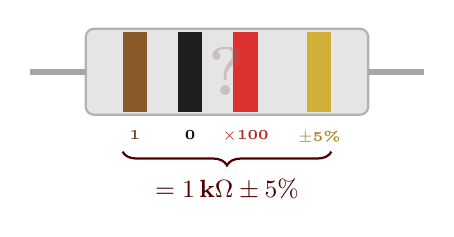
\begin{tikzpicture}[scale=0.78]
  % Resistor body
  \fill[rounded corners=3pt, fill=gray!20, draw=gray!60, line width=0.8pt]
    (-0.3,-0.7) rectangle (4.3,0.7);
  % Lead wires
  \draw[line width=2pt, gray!70] (-1.2,0) -- (-0.3,0);
  \draw[line width=2pt, gray!70] (4.3,0) -- (5.2,0);
  % Color bands
  \fill[bandbrown] (0.3,-0.65) rectangle (0.7,0.65);
  \fill[bandblack] (1.2,-0.65) rectangle (1.6,0.65);
  \fill[bandred]   (2.1,-0.65) rectangle (2.5,0.65);
  \fill[bandgold]  (3.3,-0.65) rectangle (3.7,0.65);
  % Labels
  \node[below, font=\tiny\bfseries, bandbrown!80!black] at (0.5,-0.8) {1};
  \node[below, font=\tiny\bfseries] at (1.4,-0.8) {0};
  \node[below, font=\tiny\bfseries, bandred!80!black] at (2.3,-0.8) {$\times$100};
  \node[below, font=\tiny\bfseries, bandgold!80!black] at (3.5,-0.8) {$\pm$5\%};
  % Brace
  \draw[decorate, decoration={brace, amplitude=5pt, mirror}, thick, tamumaroon]
    (0.3,-1.3) -- (3.7,-1.3)
    node[midway, below=6pt, font=\small\bfseries, tamumaroon] {$= 1\,\text{k}\Omega \pm 5\%$};
  % Question mark
  \node[font=\Huge\bfseries, tamumaroon!60, opacity=0.3] at (2,0) {?};
\end{tikzpicture}

\vspace{0.15cm}
{\scriptsize\textit{How do we automate this?}}
\end{column}
\end{columns}
\end{frame}

% ---- SLIDE: Overall System Context ----
\begin{frame}{Overall System Architecture}
\centering
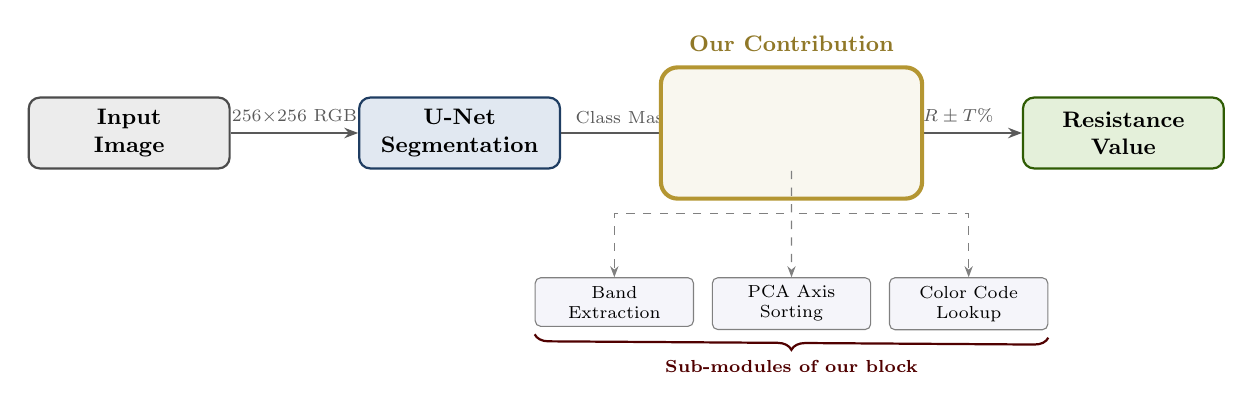
\begin{tikzpicture}[node distance=1.2cm and 1.8cm, scale=0.9, transform shape]
  % Nodes
  \node[pipeblock=gray] (input) {Input\\Image};
  \node[pipeblock=pipeblue, right=of input] (unet) {U-Net\\Segmentation};
  \node[pipeblock=pipeorange, right=of unet, draw=tamugold, line width=2pt, fill=tamugold!15] (convert) {Band Mask\\$\rightarrow$ Number};
  \node[pipeblock=pipegreen, right=of convert] (output) {Resistance\\Value};

  % Arrows
  \draw[pipearrow] (input) -- (unet) node[midway, above, font=\scriptsize] {256$\times$256 RGB};
  \draw[pipearrow] (unet) -- (convert) node[midway, above, font=\scriptsize] {Class Mask};
  \draw[pipearrow] (convert) -- (output) node[midway, above, font=\scriptsize] {$R \pm T\%$};

  % Highlight box around our contribution
  \node[fit=(convert), highlight, inner sep=10pt] (box) {};
  \node[above=2pt of box, font=\small\bfseries, tamugold!80!black] {Our Contribution};

  % Sub-steps below
  \node[databox, below=1.5cm of convert, xshift=-2.5cm] (s1) {Band\\Extraction};
  \node[databox, below=1.5cm of convert, xshift=0cm] (s2) {PCA Axis\\Sorting};
  \node[databox, below=1.5cm of convert, xshift=2.5cm] (s3) {Color Code\\Lookup};

  \draw[-{Stealth[length=4pt]}, gray, dashed] (convert.south) -- ++(0,-0.6) -| (s1.north);
  \draw[-{Stealth[length=4pt]}, gray, dashed] (convert.south) -- (s2.north);
  \draw[-{Stealth[length=4pt]}, gray, dashed] (convert.south) -- ++(0,-0.6) -| (s3.north);

  % Brace under sub-steps
  \draw[decorate, decoration={brace, amplitude=5pt, mirror}, thick, tamumaroon]
    ([yshift=-3pt]s1.south west) -- ([yshift=-3pt]s3.south east)
    node[midway, below=6pt, font=\scriptsize\bfseries, tamumaroon] {Sub-modules of our block};
\end{tikzpicture}
\end{frame}

% ============================================================================
\section{Our Contribution: Band Mask to Resistor Value}
% ============================================================================

% ---- SLIDE: Contribution Overview ----
\begin{frame}{Our Contribution --- Overview}
\small
\begin{columns}[T]
\begin{column}{0.48\textwidth}
\begin{block}{What We Built}
\small
The \textbf{Band Mask to Resistor Value} conversion block --- the complete post-segmentation pipeline that converts a pixel-level class mask into a resistance value.
\end{block}

\vspace{0.1cm}
\begin{exampleblock}{Key Modules (2,650 Lines of Python)}
\small
\begin{compactenum}
  \item \texttt{band\_extractor.py} --- 816 lines
  \item \texttt{resistance\_calculator.py} --- 460 lines
  \item \texttt{axis\_detector.py} --- 197 lines
  \item \texttt{color\_code\_tables.py} --- 229 lines
  \item \texttt{run\_inference.py} --- 470 lines
  \item \texttt{validate\_results.py} --- 267 lines
\end{compactenum}
\end{exampleblock}
\end{column}
\begin{column}{0.48\textwidth}
\begin{block}{Capabilities}
\small
\begin{compactitemize}
  \item Handles \textbf{3, 4, and 5-band} resistors
  \item Supports \textbf{arbitrary orientations} via PCA
  \item Automatic \textbf{reading direction} detection using gold tolerance band
  \item Robust \textbf{noise filtering} via connected component analysis
  \item Axis-based \textbf{majority voting} for conflicting regions
  \item \textbf{Validation framework} with E24 series checking
\end{compactitemize}
\end{block}
\end{column}
\end{columns}
\end{frame}

% ============================================================================
\section{Pipeline Architecture}
% ============================================================================

% ---- SLIDE: Detailed Pipeline Flowchart ----
\begin{frame}{Detailed Pipeline Flowchart}
\centering
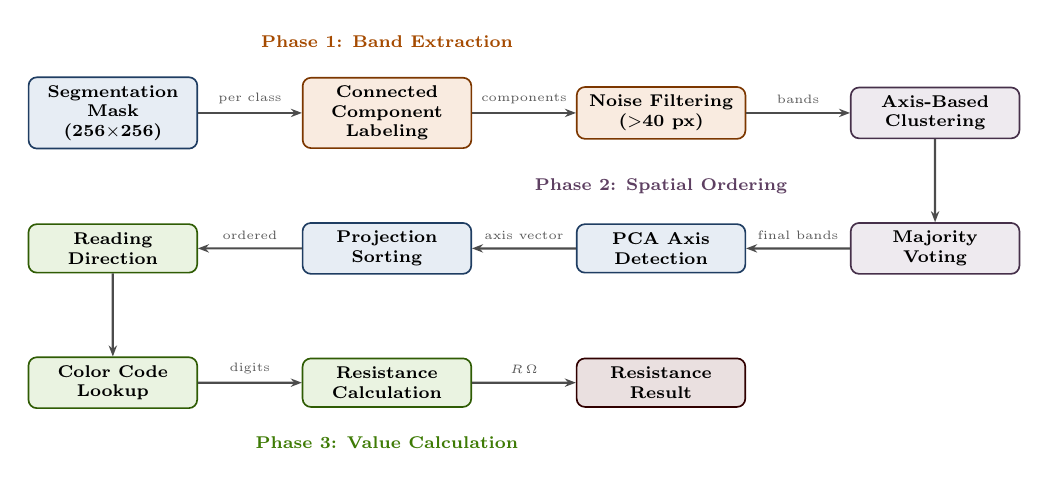
\begin{tikzpicture}[node distance=0.6cm and 0.4cm, scale=0.88, transform shape]
  % Step 1
  \node[flowblock=pipeblue] (mask) {Segmentation\\Mask (256$\times$256)};

  % Step 2
  \node[flowblock=pipeorange, right=1.5cm of mask] (ccl) {Connected\\Component\\Labeling};

  % Step 3
  \node[flowblock=pipeorange, right=1.5cm of ccl] (filter) {Noise Filtering\\($>$40 px)};

  % Step 4
  \node[flowblock=pipepurple, right=1.5cm of filter] (cluster) {Axis-Based\\Clustering};

  % Step 5 - second row
  \node[flowblock=pipepurple, below=1.2cm of cluster] (vote) {Majority\\Voting};

  % Step 6
  \node[flowblock=pipeblue, left=1.5cm of vote] (pca) {PCA Axis\\Detection};

  % Step 7
  \node[flowblock=pipeblue, left=1.5cm of pca] (sort) {Projection\\Sorting};

  % Step 8
  \node[flowblock=pipegreen, left=1.5cm of sort] (direction) {Reading\\Direction};

  % Step 9 - third row
  \node[flowblock=pipegreen, below=1.2cm of direction] (lookup) {Color Code\\Lookup};

  % Step 10
  \node[flowblock=pipegreen, right=1.5cm of lookup] (calc) {Resistance\\Calculation};

  % Step 11
  \node[flowblock=tamumaroon, right=1.5cm of calc] (result) {Resistance\\Result};

  % Arrows
  \draw[flowarrow] (mask) -- (ccl) node[midway, above, flowlabel] {per class};
  \draw[flowarrow] (ccl) -- (filter) node[midway, above, flowlabel] {components};
  \draw[flowarrow] (filter) -- (cluster) node[midway, above, flowlabel] {bands};
  \draw[flowarrow] (cluster) -- (vote);
  \draw[flowarrow] (vote) -- (pca) node[midway, above, flowlabel] {final bands};
  \draw[flowarrow] (pca) -- (sort) node[midway, above, flowlabel] {axis vector};
  \draw[flowarrow] (sort) -- (direction) node[midway, above, flowlabel] {ordered};
  \draw[flowarrow] (direction) -- (lookup);
  \draw[flowarrow] (lookup) -- (calc) node[midway, above, flowlabel] {digits};
  \draw[flowarrow] (calc) -- (result) node[midway, above, flowlabel] {$R\,\Omega$};

  % Phase labels
  \node[above=0.3cm of ccl, font=\scriptsize\bfseries, pipeorange!80!black] {Phase 1: Band Extraction};
  \node[above=0.3cm of pca, font=\scriptsize\bfseries, pipepurple!80!black] {Phase 2: Spatial Ordering};
  \node[below=0.3cm of calc, font=\scriptsize\bfseries, pipegreen!80!black] {Phase 3: Value Calculation};
\end{tikzpicture}
\end{frame}

% ---- SLIDE: Module Dependency Diagram ----
\begin{frame}{Module Architecture}
\centering
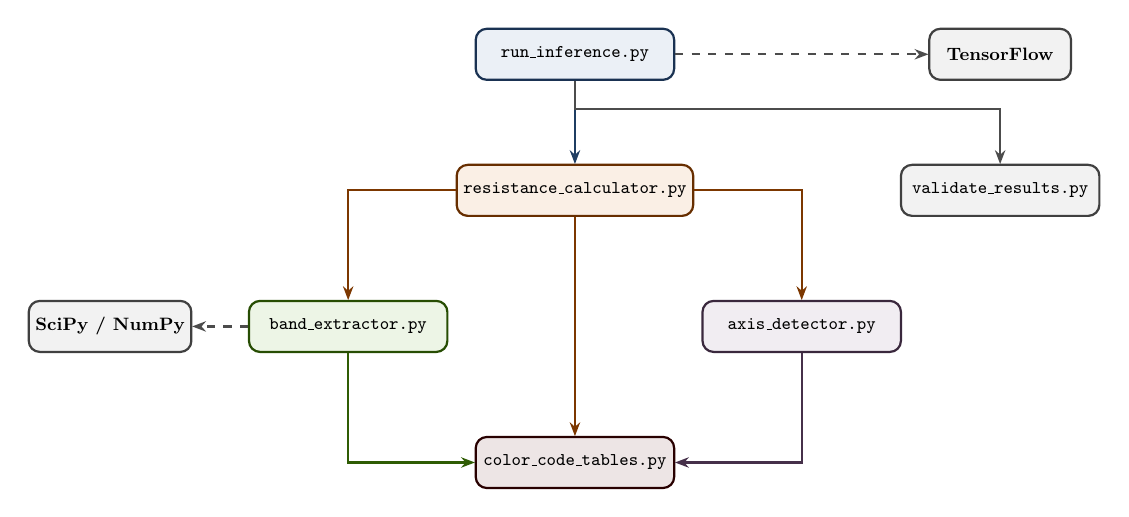
\begin{tikzpicture}[scale=0.72, transform shape]
  % Row 0: entry point + external dep (spread wide)
  \node[module=pipeblue] (run) at (0, 0) {\texttt{run\_inference.py}};
  \node[module=gray, minimum width=2.5cm] (tf) at (7.5, 0) {\textbf{TensorFlow}};

  % Row 1: orchestration layer
  \node[module=pipeorange] (calc) at (0, -2.4) {\texttt{resistance\_calculator.py}};
  \node[module=gray] (val) at (7.5, -2.4) {\texttt{validate\_results.py}};

  % Row 2: worker modules + external dep (scipy on far left)
  \node[module=gray, minimum width=2.5cm] (scipy) at (-8.2, -4.8) {SciPy / NumPy};
  \node[module=pipegreen] (band) at (-4, -4.8) {\texttt{band\_extractor.py}};
  \node[module=pipepurple] (axis) at (4, -4.8) {\texttt{axis\_detector.py}};

  % Row 3: shared data layer
  \node[module=tamumaroon] (tables) at (0, -7.2) {\texttt{color\_code\_tables.py}};

  % --- External deps (horizontal, no crossings) ---
  \draw[dep=gray, dashed] (run.east) -- (tf.west);
  \draw[dep=gray, dashed] (band.west) -- (scipy.east);

  % --- run_inference imports ---
  % run -> calc: straight down (both at x=0)
  \draw[dep=pipeblue] (run.south) -- (calc.north);
  % run -> val: down then right then down
  \draw[dep=gray] (run.south) -- ++(0,-0.5) -| (val.north);

  % --- resistance_calculator imports (separate exit points) ---
  % calc -> band: exit left edge, then down
  \draw[dep=pipeorange] (calc.west) -| (band.north);
  % calc -> axis: exit right edge, then down
  \draw[dep=pipeorange] (calc.east) -| (axis.north);
  % calc -> tables: straight down (both at x=0)
  \draw[dep=pipeorange] (calc.south) -- (tables.north);

  % --- Lower-level imports (enter tables from sides) ---
  % band -> tables: straight down then right into tables left side
  \draw[dep=pipegreen] (band.south) |- (tables.west);
  % axis -> tables: straight down then left into tables right side
  \draw[dep=pipepurple] (axis.south) |- (tables.east);
\end{tikzpicture}
\end{frame}

% ============================================================================
\section{Algorithm Details}
% ============================================================================

% ---- SLIDE: Band Extraction Algorithm ----
\begin{frame}[fragile]{Step 1: Band Extraction via Connected Component Analysis}
\begin{columns}[T]
\begin{column}{0.52\textwidth}
\begin{block}{Algorithm}
\small
For each color class $c \in \{1,\ldots,12\} \setminus \{0,5\}$:
\begin{compactenum}
  \item Binary mask: $M_c[i,j] = \mathbf{1}[\text{mask}[i,j] = c]$
  \item Apply \texttt{scipy.ndimage.label()} (8-connectivity)
  \item Per component $k$: compute centroid, area $A_k$, bounding box
  \item \textbf{Filter}: Discard if $A_k < 40$ pixels
  \item \textbf{Merge}: Combine nearby same-color fragments ($<$15\,px)
\end{compactenum}
\end{block}
\end{column}
\begin{column}{0.44\textwidth}
\centering
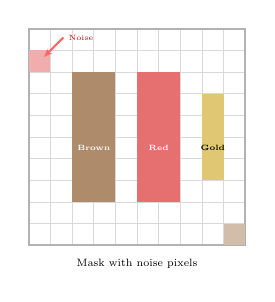
\begin{tikzpicture}[scale=0.55, transform shape]
  % Grid representing mask
  \draw[step=0.5, gray!30, very thin] (0,0) grid (5,5);
  \draw[thick, gray!60] (0,0) rectangle (5,5);

  % Brown band region (manual instead of foreach)
  \fill[bandbrown!70] (1,1) rectangle ++(0.5,0.5);
  \fill[bandbrown!70] (1,1.5) rectangle ++(0.5,0.5);
  \fill[bandbrown!70] (1,2) rectangle ++(0.5,0.5);
  \fill[bandbrown!70] (1,2.5) rectangle ++(0.5,0.5);
  \fill[bandbrown!70] (1,3) rectangle ++(0.5,0.5);
  \fill[bandbrown!70] (1,3.5) rectangle ++(0.5,0.5);
  \fill[bandbrown!70] (1.5,1) rectangle ++(0.5,0.5);
  \fill[bandbrown!70] (1.5,1.5) rectangle ++(0.5,0.5);
  \fill[bandbrown!70] (1.5,2) rectangle ++(0.5,0.5);
  \fill[bandbrown!70] (1.5,2.5) rectangle ++(0.5,0.5);
  \fill[bandbrown!70] (1.5,3) rectangle ++(0.5,0.5);
  \fill[bandbrown!70] (1.5,3.5) rectangle ++(0.5,0.5);

  % Red band region
  \fill[bandred!70] (2.5,1) rectangle ++(0.5,0.5);
  \fill[bandred!70] (2.5,1.5) rectangle ++(0.5,0.5);
  \fill[bandred!70] (2.5,2) rectangle ++(0.5,0.5);
  \fill[bandred!70] (2.5,2.5) rectangle ++(0.5,0.5);
  \fill[bandred!70] (2.5,3) rectangle ++(0.5,0.5);
  \fill[bandred!70] (2.5,3.5) rectangle ++(0.5,0.5);
  \fill[bandred!70] (3,1) rectangle ++(0.5,0.5);
  \fill[bandred!70] (3,1.5) rectangle ++(0.5,0.5);
  \fill[bandred!70] (3,2) rectangle ++(0.5,0.5);
  \fill[bandred!70] (3,2.5) rectangle ++(0.5,0.5);
  \fill[bandred!70] (3,3) rectangle ++(0.5,0.5);
  \fill[bandred!70] (3,3.5) rectangle ++(0.5,0.5);

  % Gold band region
  \fill[bandgold!70] (4,1.5) rectangle ++(0.5,0.5);
  \fill[bandgold!70] (4,2) rectangle ++(0.5,0.5);
  \fill[bandgold!70] (4,2.5) rectangle ++(0.5,0.5);
  \fill[bandgold!70] (4,3) rectangle ++(0.5,0.5);

  % Noise pixels
  \fill[bandred!40] (0,4) rectangle ++(0.5,0.5);
  \fill[bandbrown!40] (4.5,0) rectangle ++(0.5,0.5);

  % Labels
  \node[font=\tiny\bfseries, white] at (1.5,2.25) {Brown};
  \node[font=\tiny\bfseries, white] at (3,2.25) {Red};
  \node[font=\tiny\bfseries] at (4.25,2.25) {\tiny Gold};

  % Noise label
  \draw[-{Stealth[length=3pt]}, red!60, thick] (0.8,4.8) -- (0.35,4.35);
  \node[font=\tiny, red!70!black, right] at (0.8,4.8) {Noise};

  % Caption
  \node[below=0.2cm, font=\scriptsize] at (2.5,0) {Mask with noise pixels};
\end{tikzpicture}

\vspace{0.1cm}
{\scriptsize CCL separates bands from noise; area filtering removes artifacts.}
\end{column}
\end{columns}
\end{frame}

% ---- SLIDE: PCA Axis Detection ----
\begin{frame}{Step 2: PCA-Based Axis Detection \& Sorting}
\begin{columns}[T]
\begin{column}{0.50\textwidth}
\begin{block}{PCA Algorithm}
\small
Given centroids $\{\mathbf{p}_1, \ldots, \mathbf{p}_n\}$:
\begin{compactenum}
  \item Center: $\bar{\mathbf{p}} = \frac{1}{n}\sum_i \mathbf{p}_i$
  \item Covariance: $\boldsymbol{\Sigma} = \frac{1}{n}\mathbf{X}^T\mathbf{X}$
  \item Eigendecomposition: $\boldsymbol{\Sigma}\mathbf{v} = \lambda \mathbf{v}$
  \item Principal axis: $\hat{\mathbf{v}} = \text{eigvec}(\max \lambda)$
\end{compactenum}
\end{block}

\vspace{0.1cm}
\begin{block}{Projection Sorting}
For each band $i$, compute scalar projection:
\[
  s_i = (\mathbf{p}_i - \bar{\mathbf{p}}) \cdot \hat{\mathbf{v}}
\]
Sort bands by $s_i$ to obtain left-to-right order.
\end{block}
\end{column}
\begin{column}{0.46\textwidth}
\centering
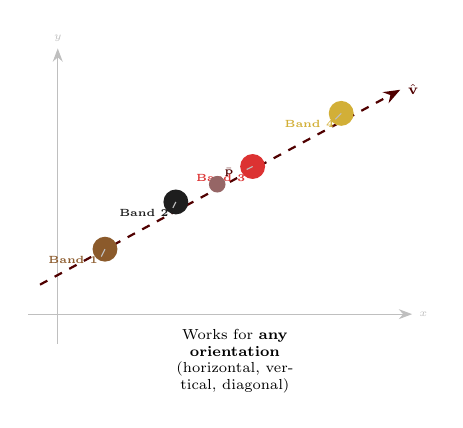
\begin{tikzpicture}[scale=0.75, transform shape]
  % Coordinate system
  \draw[-{Stealth}, gray!50] (-0.5,0) -- (6,0) node[right, font=\tiny] {$x$};
  \draw[-{Stealth}, gray!50] (0,-0.5) -- (0,4.5) node[above, font=\tiny] {$y$};

  % PCA axis (diagonal)
  \draw[thick, tamumaroon, dashed, -{Stealth[length=6pt]}] (-0.3,0.5) -- (5.8,3.8)
    node[right, font=\scriptsize\bfseries, tamumaroon] {$\hat{\mathbf{v}}$};

  % Band centroids (along diagonal with slight offset)
  \fill[bandbrown] (0.8,1.1) circle (6pt) node[below left, font=\tiny\bfseries] {Band 1};
  \fill[bandblack] (2.0,1.9) circle (6pt) node[below left, font=\tiny\bfseries] {Band 2};
  \fill[bandred] (3.3,2.5) circle (6pt) node[below left, font=\tiny\bfseries] {Band 3};
  \fill[bandgold] (4.8,3.4) circle (6pt) node[below left, font=\tiny\bfseries] {Band 4};

  % Projections onto axis
  \draw[thin, gray!50, dashed] (0.8,1.1) -- (0.7,0.9);
  \draw[thin, gray!50, dashed] (2.0,1.9) -- (1.95,1.8);
  \draw[thin, gray!50, dashed] (3.3,2.5) -- (3.2,2.45);
  \draw[thin, gray!50, dashed] (4.8,3.4) -- (4.7,3.3);

  % Mean point
  \fill[tamumaroon!60] (2.7,2.2) circle (4pt);
  \node[font=\tiny, tamumaroon, above right] at (2.7,2.2) {$\bar{\mathbf{p}}$};

  % Annotation
  \node[font=\scriptsize, text width=3cm, align=center] at (3,-0.8)
    {Works for \textbf{any orientation}\\(horizontal, vertical, diagonal)};
\end{tikzpicture}
\end{column}
\end{columns}
\end{frame}

% ---- SLIDE: Reading Direction ----
\begin{frame}{Step 3: Reading Direction Detection}
\centering
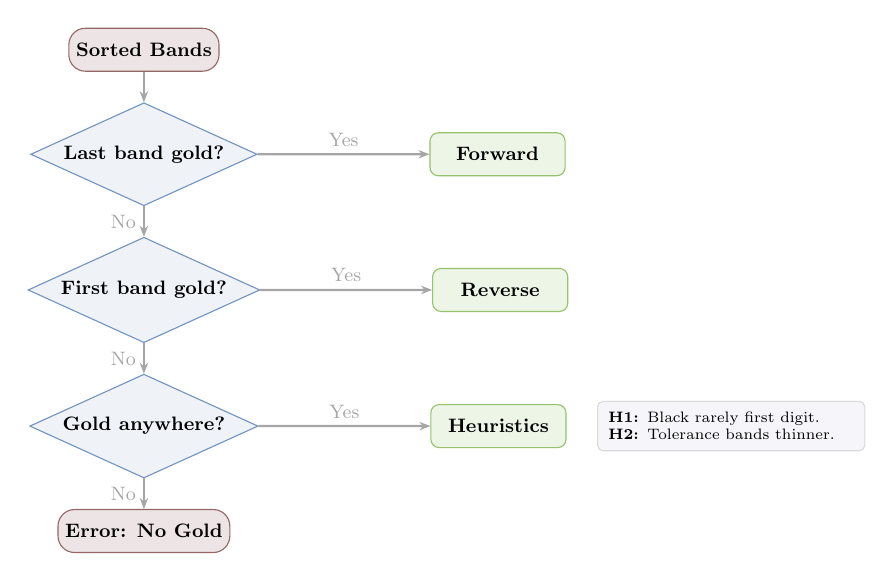
\begin{tikzpicture}[node distance=0.5cm, scale=0.78, transform shape,
  smalldiamond/.style={diamond, aspect=2.2, draw=pipeblue!70, fill=pipeblue!8,
    text centered, font=\small\bfseries, inner sep=2pt, minimum width=2.8cm},
  smallprocess/.style={rectangle, rounded corners=3pt, draw=pipegreen!60, fill=pipegreen!10,
    text centered, font=\small\bfseries, minimum width=2.2cm, minimum height=0.7cm},
  smallstop/.style={rectangle, rounded corners=6pt, draw=tamumaroon!60, fill=tamumaroon!10,
    text centered, font=\small\bfseries, minimum width=2.2cm, minimum height=0.7cm}
]
  % Start
  \node[smallstop] (start) {Sorted Bands};

  % Decision 1
  \node[smalldiamond, below=0.5cm of start] (d1) {Last band gold?};

  % Yes -> forward
  \node[smallprocess, right=2.8cm of d1] (forward) {Forward};

  % Decision 2
  \node[smalldiamond, below=0.5cm of d1] (d2) {First band gold?};

  % Yes -> reverse
  \node[smallprocess, right=2.8cm of d2] (reverse) {Reverse};

  % Decision 3
  \node[smalldiamond, below=0.5cm of d2] (d3) {Gold anywhere?};

  % Yes -> heuristics
  \node[smallprocess, right=2.8cm of d3] (heur) {Heuristics};

  % No -> error
  \node[smallstop, below=0.5cm of d3] (error) {Error: No Gold};

  % Arrows
  \draw[decarrow] (start) -- (d1);
  \draw[decarrow] (d1) -- (forward) node[midway, above, font=\small] {Yes};
  \draw[decarrow] (d1) -- (d2) node[midway, left, font=\small] {No};
  \draw[decarrow] (d2) -- (reverse) node[midway, above, font=\small] {Yes};
  \draw[decarrow] (d2) -- (d3) node[midway, left, font=\small] {No};
  \draw[decarrow] (d3) -- (heur) node[midway, above, font=\small] {Yes};
  \draw[decarrow] (d3) -- (error) node[midway, left, font=\small] {No};

  % Heuristics detail box
  \node[right=0.5cm of heur, text width=4cm, font=\scriptsize, align=left, draw=gray!30, fill=lightbg, rounded corners=2pt, inner sep=5pt] {
    \textbf{H1:} Black rarely first digit.
    \textbf{H2:} Tolerance bands thinner.
  };
\end{tikzpicture}
\end{frame}

% ---- SLIDE: Resistance Calculation ----
\begin{frame}{Step 4: Resistance Value Calculation}
\begin{columns}[T]
\begin{column}{0.48\textwidth}
\begin{block}{4-Band Resistor}
\centering
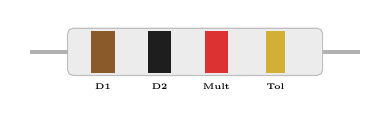
\begin{tikzpicture}[scale=0.6, transform shape]
  \fill[rounded corners=2pt, gray!15, draw=gray!50] (-0.2,-0.5) rectangle (5.2,0.5);
  \draw[line width=1.5pt, gray!60] (-1,0) -- (-0.2,0);
  \draw[line width=1.5pt, gray!60] (5.2,0) -- (6,0);
  \fill[bandbrown] (0.3,-0.45) rectangle (0.8,0.45);
  \fill[bandblack] (1.5,-0.45) rectangle (2.0,0.45);
  \fill[bandred]   (2.7,-0.45) rectangle (3.2,0.45);
  \fill[bandgold]  (4.0,-0.45) rectangle (4.4,0.45);
  \node[below, font=\tiny\bfseries] at (0.55,-0.55) {D1};
  \node[below, font=\tiny\bfseries] at (1.75,-0.55) {D2};
  \node[below, font=\tiny\bfseries] at (2.95,-0.55) {Mult};
  \node[below, font=\tiny\bfseries] at (4.2,-0.55) {Tol};
\end{tikzpicture}
\vspace{0.1cm}
\[ R = (D_1 \times 10 + D_2) \times \text{Mult} \]
\small\textbf{Ex:} Brown--Black--Red--Gold\\
$R = (1 \times 10 + 0) \times 100 = 1\,\text{k}\Omega \pm 5\%$
\end{block}
\end{column}
\begin{column}{0.48\textwidth}
\begin{block}{5-Band Resistor (Precision)}
\centering
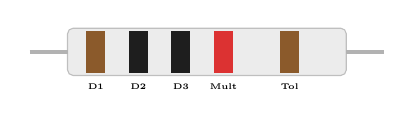
\begin{tikzpicture}[scale=0.6, transform shape]
  \fill[rounded corners=2pt, gray!15, draw=gray!50] (-0.2,-0.5) rectangle (5.7,0.5);
  \draw[line width=1.5pt, gray!60] (-1,0) -- (-0.2,0);
  \draw[line width=1.5pt, gray!60] (5.7,0) -- (6.5,0);
  \fill[bandbrown] (0.2,-0.45) rectangle (0.6,0.45);
  \fill[bandblack] (1.1,-0.45) rectangle (1.5,0.45);
  \fill[bandblack] (2.0,-0.45) rectangle (2.4,0.45);
  \fill[bandred]   (2.9,-0.45) rectangle (3.3,0.45);
  \fill[bandbrown] (4.3,-0.45) rectangle (4.7,0.45);
  \node[below, font=\tiny\bfseries] at (0.4,-0.55) {D1};
  \node[below, font=\tiny\bfseries] at (1.3,-0.55) {D2};
  \node[below, font=\tiny\bfseries] at (2.2,-0.55) {D3};
  \node[below, font=\tiny\bfseries] at (3.1,-0.55) {Mult};
  \node[below, font=\tiny\bfseries] at (4.5,-0.55) {Tol};
\end{tikzpicture}
\vspace{0.1cm}
\[ R = (D_1 \times 100 + D_2 \times 10 + D_3) \times \text{Mult} \]
\small\textbf{Ex:} Brown--Black--Black--Red--Brown\\
$R = (100 + 0 + 0) \times 100 = 10\,\text{k}\Omega \pm 1\%$
\end{block}
\end{column}
\end{columns}

\vspace{0.1cm}
\centering
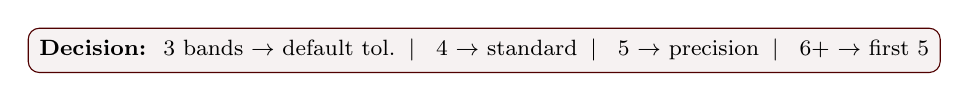
\begin{tikzpicture}
\node[draw=tamumaroon, rounded corners=4pt, fill=tamumaroon!5, inner sep=4pt, font=\footnotesize] {
  \textbf{Decision:}\;
  3 bands $\rightarrow$ default tol.\;\;$|$\;\;
  4 $\rightarrow$ standard\;\;$|$\;\;
  5 $\rightarrow$ precision\;\;$|$\;\;
  6+ $\rightarrow$ first 5
};
\end{tikzpicture}
\end{frame}

% ============================================================================
\section{Color Code Mapping}
% ============================================================================

% ---- SLIDE: Color Code Table ----
\begin{frame}{Resistor Color Code Reference}
\centering
\small
\renewcommand{\arraystretch}{1.15}
\begin{tabular}{>{\centering}m{1.2cm} c c c c}
\toprule
\textbf{Color} & \textbf{Class ID} & \textbf{Digit} & \textbf{Multiplier} & \textbf{Tolerance} \\
\midrule
\cellcolor{bandblack!80}\textcolor{white}{\textbf{Black}} & 8 & 0 & $\times 1$ & --- \\
\cellcolor{bandbrown!70}\textcolor{white}{\textbf{Brown}} & 4 & 1 & $\times 10$ & $\pm 1\%$ \\
\cellcolor{bandred!70}\textcolor{white}{\textbf{Red}} & 11 & 2 & $\times 100$ & $\pm 2\%$ \\
\cellcolor{bandorange!70}\textbf{Orange} & 2 & 3 & $\times 1\text{k}$ & --- \\
\cellcolor{bandyellow!70}\textbf{Yellow} & 7 & 4 & $\times 10\text{k}$ & --- \\
\cellcolor{bandgreen!70}\textcolor{white}{\textbf{Green}} & 3 & 5 & $\times 100\text{k}$ & $\pm 0.5\%$ \\
\cellcolor{bandblue!70}\textcolor{white}{\textbf{Blue}} & 6 & 6 & $\times 1\text{M}$ & $\pm 0.25\%$ \\
\cellcolor{bandviolet!70}\textcolor{white}{\textbf{Violet}} & 12 & 7 & $\times 10\text{M}$ & $\pm 0.1\%$ \\
\cellcolor{bandgrey!70}\textbf{Grey} & 10 & 8 & $\times 100\text{M}$ & $\pm 0.05\%$ \\
\cellcolor{bandwhite}\textbf{White} & 9 & 9 & $\times 1\text{G}$ & --- \\
\cellcolor{bandgold!70}\textbf{Gold} & 1 & --- & $\times 0.1$ & $\pm 5\%$ \\
\bottomrule
\end{tabular}

\vspace{0.3cm}
{\footnotesize \textbf{Note:} The U-Net model outputs 13 classes --- 11 colors + 2 background classes (image background \& resistor body).}
\end{frame}

% ============================================================================
\section{Data Structures}
% ============================================================================

% ---- SLIDE: Data Structures ----
\begin{frame}[fragile]{Core Data Structures}
\begin{columns}[T]
\begin{column}{0.48\textwidth}
\begin{block}{\texttt{BandInfo}}
\begin{lstlisting}[language=Python]
@dataclass
class BandInfo:
    class_id: int        # 0-12
    color_name: str      # "brown"
    centroid: (float,float)
    area: int
    bounding_box: (int,int,int,int)
\end{lstlisting}
\end{block}
\vspace{0.05cm}
\begin{block}{\texttt{ResistanceResult}}
\begin{lstlisting}[language=Python]
@dataclass
class ResistanceResult:
    value: float      # e.g. 1000.0
    tolerance: float  # e.g. 5.0
    band_count: int   # 3, 4, or 5
    bands: List[BandInfo]
\end{lstlisting}
\end{block}
\end{column}
\begin{column}{0.48\textwidth}
\begin{block}{\texttt{CalculationError}}
\begin{lstlisting}[language=Python]
@dataclass
class CalculationError:
    error_type: str
    message: str
    detected_bands: List[BandInfo]
\end{lstlisting}
\end{block}
\vspace{0.05cm}
\begin{block}{Lookup Tables}
\begin{lstlisting}[language=Python]
COLOR_TO_DIGIT = {
  "black":0, "brown":1, "red":2,
  "orange":3, "yellow":4,
  "green":5, "blue":6, "violet":7,
  "grey":8, "white":9 }
COLOR_TO_MULTIPLIER = {
  "black":1, "brown":10,
  "red":100, "orange":1e3, ... }
\end{lstlisting}
\end{block}
\end{column}
\end{columns}
\end{frame}

% ============================================================================
\section{End-to-End Walkthrough}
% ============================================================================

% ---- SLIDE: Worked Example ----
\begin{frame}{Worked Example: 1\,k$\Omega$ Resistor}
\centering
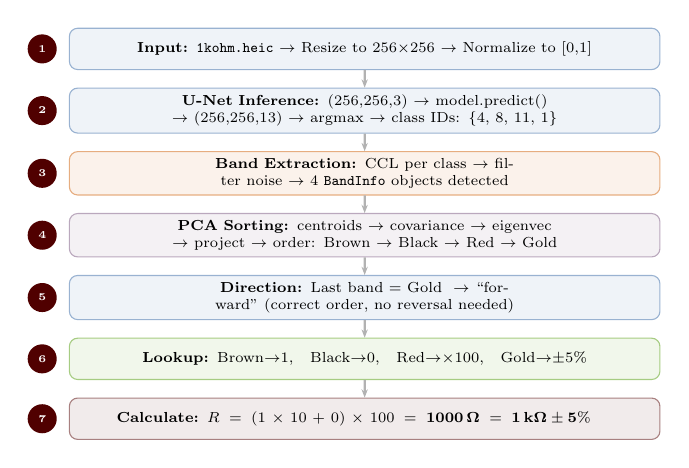
\begin{tikzpicture}[node distance=0.5cm, scale=0.75, transform shape]
  \node[stepbox=pipeblue] (s1) {
    \textbf{Input:} \texttt{1kohm.heic} $\rightarrow$ Resize to 256$\times$256 $\rightarrow$ Normalize to [0,1]
  };
  \node[stepnum, left=0.2cm of s1] {1};

  \node[stepbox=pipeblue, below=0.3cm of s1] (s2) {
    \textbf{U-Net Inference:} (256,256,3) $\rightarrow$ model.predict() $\rightarrow$ (256,256,13) $\rightarrow$ argmax $\rightarrow$ class IDs: \{4, 8, 11, 1\}
  };
  \node[stepnum, left=0.2cm of s2] {2};

  \node[stepbox=pipeorange, below=0.3cm of s2] (s3) {
    \textbf{Band Extraction:} CCL per class $\rightarrow$ filter noise $\rightarrow$ 4 \texttt{BandInfo} objects detected
  };
  \node[stepnum, left=0.2cm of s3] {3};

  \node[stepbox=pipepurple, below=0.3cm of s3] (s4) {
    \textbf{PCA Sorting:} centroids $\rightarrow$ covariance $\rightarrow$ eigenvec $\rightarrow$ project $\rightarrow$ order: Brown $\rightarrow$ Black $\rightarrow$ Red $\rightarrow$ Gold
  };
  \node[stepnum, left=0.2cm of s4] {4};

  \node[stepbox=pipeblue, below=0.3cm of s4] (s5) {
    \textbf{Direction:} Last band = Gold $\checkmark$ $\rightarrow$ ``forward'' (correct order, no reversal needed)
  };
  \node[stepnum, left=0.2cm of s5] {5};

  \node[stepbox=pipegreen, below=0.3cm of s5] (s6) {
    \textbf{Lookup:} Brown$\rightarrow$1,\quad Black$\rightarrow$0,\quad Red$\rightarrow$$\times$100,\quad Gold$\rightarrow$$\pm$5\%
  };
  \node[stepnum, left=0.2cm of s6] {6};

  \node[stepbox=tamumaroon, below=0.3cm of s6] (s7) {
    \textbf{Calculate:} $R = (1 \times 10 + 0) \times 100 = \mathbf{1000\,\Omega} = \mathbf{1\,k\Omega \pm 5\%}$ \quad $\checkmark$
  };
  \node[stepnum, left=0.2cm of s7] {7};

  % Arrows (manual instead of foreach)
  \draw[steparrow] (s1) -- (s2);
  \draw[steparrow] (s2) -- (s3);
  \draw[steparrow] (s3) -- (s4);
  \draw[steparrow] (s4) -- (s5);
  \draw[steparrow] (s5) -- (s6);
  \draw[steparrow] (s6) -- (s7);
\end{tikzpicture}
\end{frame}

% ============================================================================
\section{Results \& Validation}
% ============================================================================

% ---- SLIDE: Results ----
\begin{frame}{Results \& Performance}
\small
\begin{columns}[T]
\begin{column}{0.48\textwidth}
\begin{block}{Test Dataset}
\scriptsize
\begin{compactitemize}
  \item \textbf{45 resistor images} (HEIC, JPG, PNG)
  \item Range: $1\,\Omega$ to $1\,\text{M}\Omega$
  \item Various orientations and lighting
  \item 9 validation runs performed
\end{compactitemize}
\end{block}

\vspace{0.05cm}
\begin{exampleblock}{Overall Accuracy}
\centering
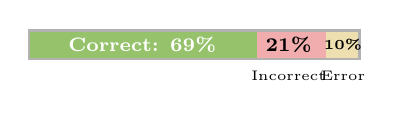
\begin{tikzpicture}[scale=0.6]
  \fill[pipegreen!60] (0,0) rectangle (4.83,0.6);
  \fill[bandred!40] (4.83,0) rectangle (6.3,0.6);
  \fill[bandgold!40] (6.3,0) rectangle (7,0.6);
  \draw[thick, gray!60] (0,0) rectangle (7,0.6);
  \node[font=\scriptsize\bfseries, white] at (2.4,0.3) {Correct: 69\%};
  \node[font=\scriptsize\bfseries] at (5.5,0.3) {21\%};
  \node[font=\tiny\bfseries] at (6.65,0.3) {10\%};
  \node[below, font=\tiny] at (5.5,-0.05) {Incorrect};
  \node[below, font=\tiny] at (6.65,-0.05) {Error};
\end{tikzpicture}
\end{exampleblock}

\vspace{0.05cm}
\begin{alertblock}{Error Sources}
\scriptsize
\begin{compactitemize}
  \item Color confusion (green/grey, brown/black)
  \item Light reflection mistaken for grey
  \item Small artifacts mistaken for full bands
\end{compactitemize}
\end{alertblock}
\end{column}
\begin{column}{0.48\textwidth}
\begin{block}{Performance Metrics}
\scriptsize
\renewcommand{\arraystretch}{1.0}
\begin{tabular}{l r}
\toprule
\textbf{Metric} & \textbf{Value} \\
\midrule
Images Tested & 42 \\
Correct & 29 (69\%) \\
Incorrect & 9 (21\%) \\
Errors & 4 (10\%) \\
\midrule
Inference Time & $\sim$0.5--1\,s \\
Post-processing & $\sim$10\,ms \\
Model Memory & $\sim$90\,MB \\
\bottomrule
\end{tabular}
\end{block}
\end{column}
\end{columns}
\end{frame}

% ---- SLIDE: Case Study ----
\begin{frame}{Case Study: Correct vs.\ Incorrect Conversion}
\begin{columns}[T]
\begin{column}{0.48\textwidth}
\begin{exampleblock}{Correct: 10\,k$\Omega$ Resistor}
\centering
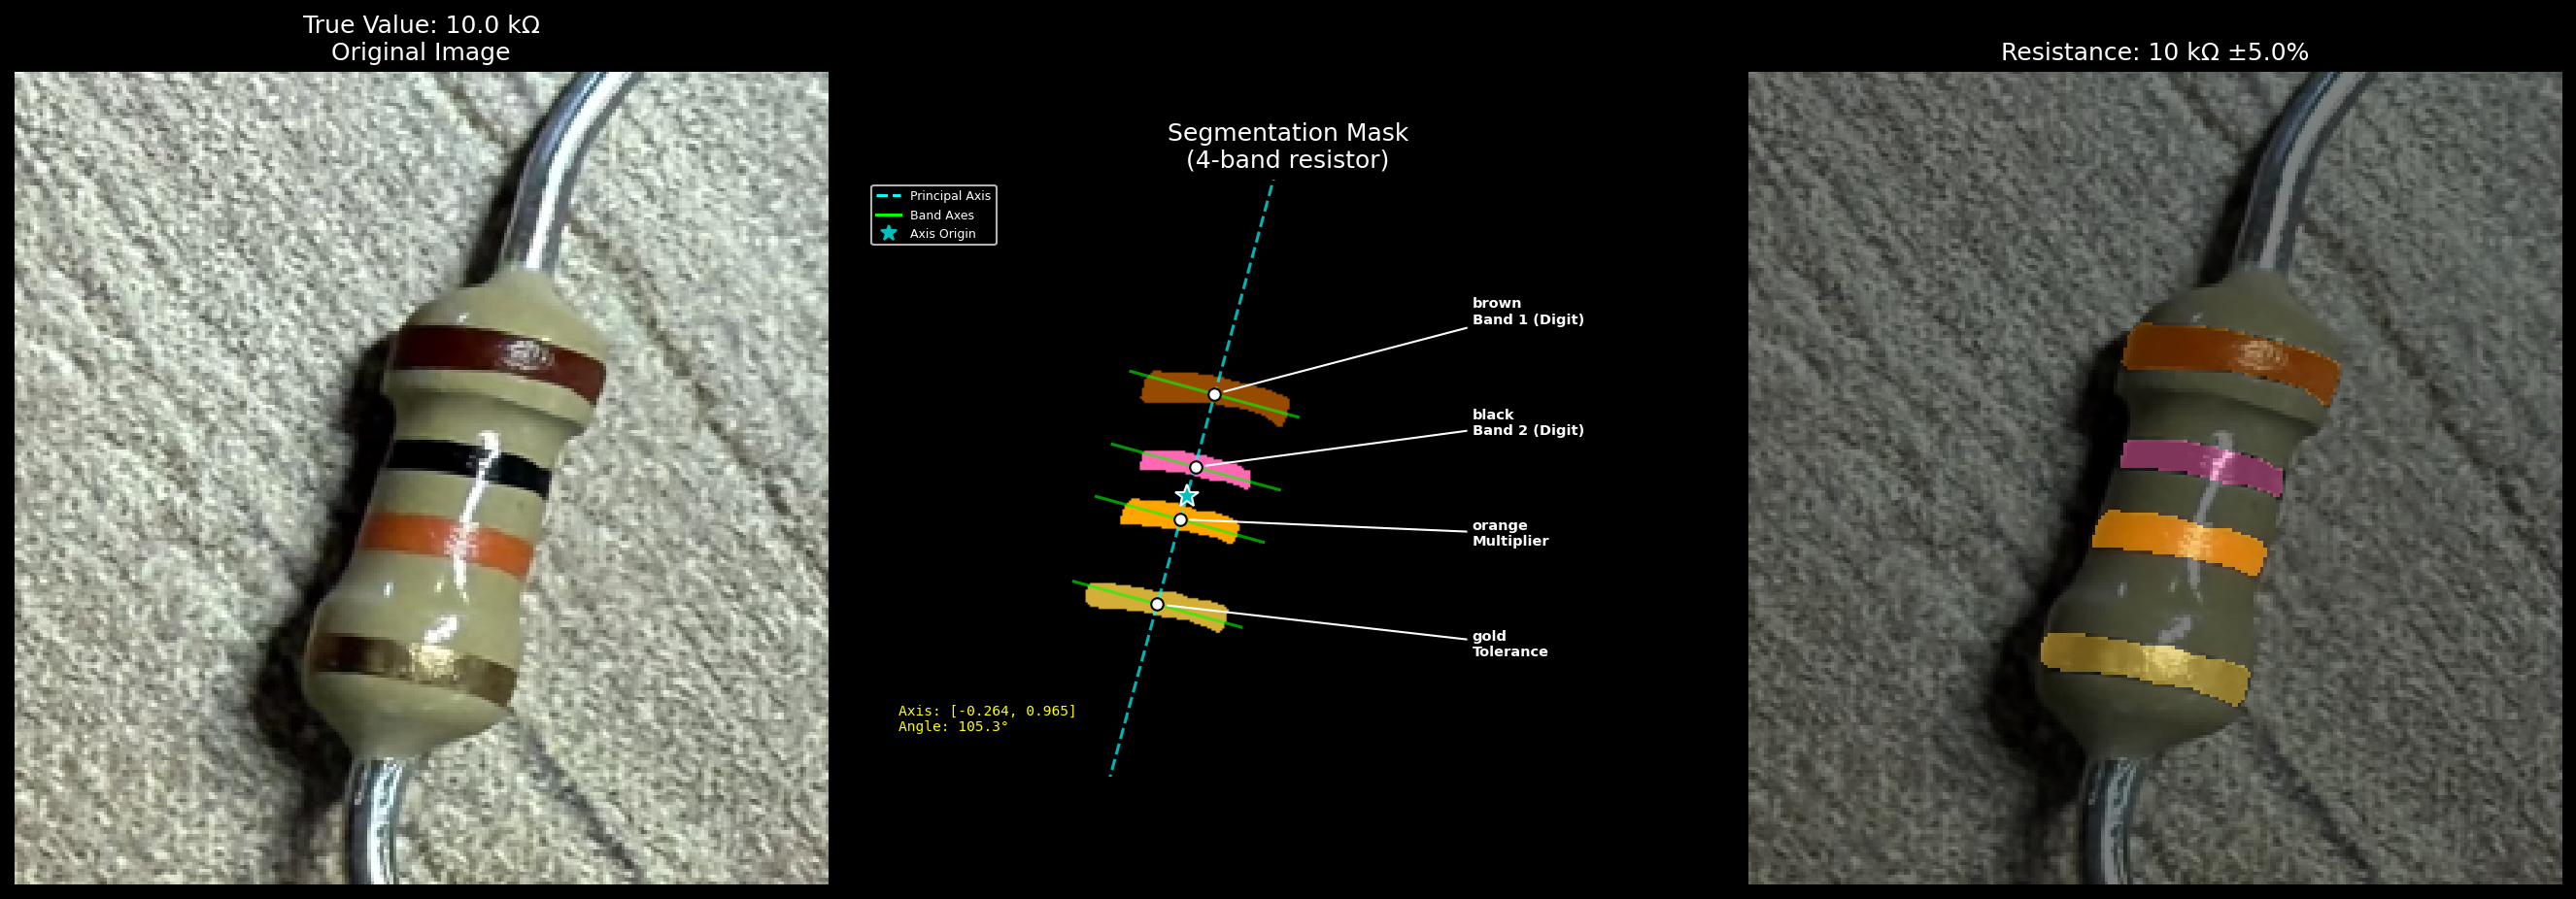
\includegraphics[width=\textwidth]{case_correct.png}
\vspace{0.1cm}

\scriptsize
\renewcommand{\arraystretch}{1.0}
\begin{tabular}{l l}
\textbf{True Value:} & 10.0\,k$\Omega$ \\
\textbf{Detected:} & Brown--Black--Orange--Gold \\
\textbf{Calculated:} & $(1{\times}10{+}0){\times}1000 = 10$\,k$\Omega$ \\
\textbf{Status:} & \textcolor{pipegreen}{\textbf{Correct (0\% error)}}
\end{tabular}
\end{exampleblock}
\end{column}
\begin{column}{0.48\textwidth}
\begin{alertblock}{Incorrect: 220\,$\Omega$ Resistor}
\centering
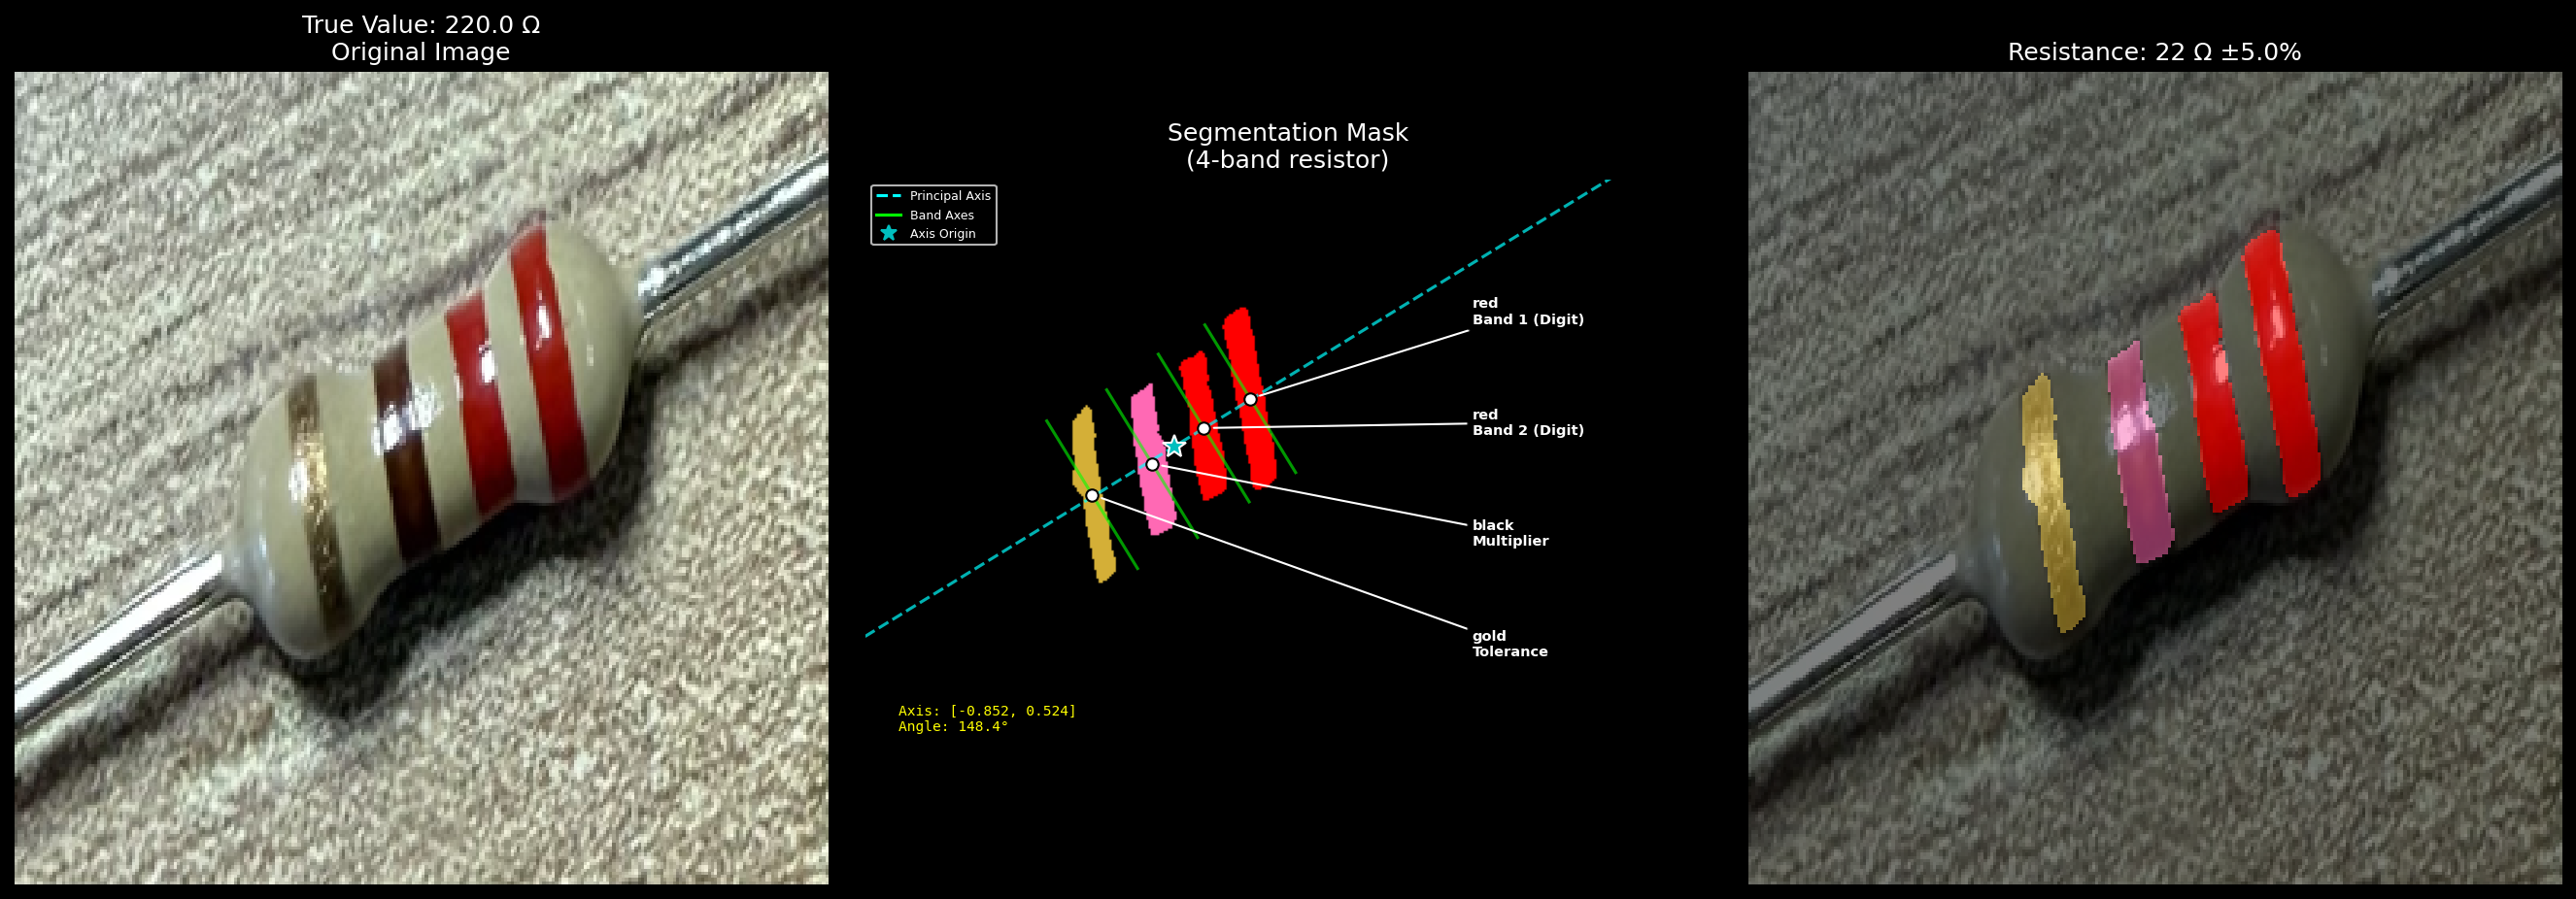
\includegraphics[width=\textwidth]{case_incorrect.png}
\vspace{0.1cm}

\scriptsize
\renewcommand{\arraystretch}{1.0}
\begin{tabular}{l l}
\textbf{True Value:} & 220\,$\Omega$ \\
\textbf{Expected:} & Red--Red--Brown--Gold \\
\textbf{Detected:} & Red--Red--Black--Gold \\
\textbf{Calculated:} & $(2{\times}10{+}2){\times}1 = 22$\,$\Omega$ \\
\textbf{Status:} & \textcolor{bandred}{\textbf{Incorrect (90\% error)}}
\end{tabular}

\vspace{0.1cm}
\scriptsize\textbf{Root cause:} Brown multiplier band misclassified as black (${\times}1$ instead of ${\times}10$)
\end{alertblock}
\end{column}
\end{columns}
\end{frame}

% ============================================================================
\section{Robustness Features}
% ============================================================================

% ---- SLIDE: Robustness ----
\begin{frame}{Robustness \& Edge Case Handling}
\small
\begin{columns}[T]
\begin{column}{0.48\textwidth}
\begin{block}{Noise Rejection}
\small
\begin{compactitemize}
  \item \textbf{Area filtering}: Components $<$40\,px discarded
  \item \textbf{Component merging}: Same-color fragments merged ($<$15\,px)
  \item \textbf{Band cap}: If $>$6 detected, keep top-5 by area
\end{compactitemize}
\end{block}
\vspace{0.05cm}
\begin{block}{Orientation Invariance}
\small
\begin{compactitemize}
  \item PCA handles \textbf{any angle}
  \item No horizontal/vertical assumption
  \item Works with $\geq$2 centroids
\end{compactitemize}
\end{block}
\end{column}
\begin{column}{0.48\textwidth}
\begin{block}{Axis-Based Majority Voting}
\small
\begin{compactitemize}
  \item When colors overlap same axis position:
  \begin{compactenum}
    \item Cluster by perpendicular distance ($<$15\,px)
    \item Largest total area wins
  \end{compactenum}
  \item Resolves ambiguous segmentation
\end{compactitemize}
\end{block}
\vspace{0.05cm}
\begin{block}{Validation Checks}
\small
\begin{compactitemize}
  \item E24 standard series validation
  \item Range: $0.1\,\Omega$ -- $100\,\text{M}\Omega$
  \item Color validity per band position
\end{compactitemize}
\end{block}
\end{column}
\end{columns}
\end{frame}

% ---- SLIDE: Fine-Tuneable Parameters ----
\begin{frame}{Fine-Tuneable Parameters}
\centering
\resizebox{\textwidth}{!}{%
\scriptsize
\renewcommand{\arraystretch}{1.25}
\begin{tabular}{l c l l}
\toprule
\textbf{Parameter} & \textbf{Value} & \textbf{Purpose} & \textbf{Justification} \\
\midrule
\texttt{MIN\_BAND\_AREA} & 40\,px & Min.\ pixels for a valid band & Filters noise; tested vs.\ 50\,px \\
\texttt{MERGE\_DISTANCE} & 10\,px & Max.\ centroid gap to merge fragments & Reunites splits without merging neighbors \\
\texttt{BAND\_AXIS\_THRESH} & 15\,px & Perpendicular distance for axis grouping & Tolerates slight segmentation offset \\
\texttt{MAX\_BANDS\_TRIGGER} & 6 & Band count to trigger area filter & 5-band max + 1 noise tolerance \\
\texttt{MAX\_BANDS\_KEPT} & 5 & Bands kept after filtering & Matches 5-band precision resistor \\
\texttt{MIN\_BAND\_COUNT} & 3 & Min.\ bands for calculation & 2 digits + 1 multiplier minimum \\
\texttt{WIDTH\_RATIO} & 0.7 & Width ratio for direction heuristic & Tolerance bands typically ${<}$70\% of digit width \\
\texttt{DEFAULT\_TOL} & 20\% & Fallback when no tolerance band found & Standard for 3-band resistors \\
\texttt{INPUT\_SIZE} & 256${\times}$256 & Image preprocessing resolution & U-Net training resolution \\
\texttt{VALIDATION\_TOL} & 10\% & Error threshold for ``correct'' label & Covers E24 rounding \& measurement drift \\
\bottomrule
\end{tabular}%
}

\vspace{0.15cm}

\begin{tikzpicture}
\node[draw=tamugold, rounded corners=4pt, fill=tamugold!8, inner sep=4pt, font=\scriptsize] {
  All values empirically chosen on 45-image dataset --- grid search could improve accuracy.
};
\end{tikzpicture}
\end{frame}

% ============================================================================
\section{Limitations \& Future Work}
% ============================================================================

% ---- SLIDE: Limitations ----
\begin{frame}{Limitations \& Future Work}
\small
\begin{columns}[T]
\begin{column}{0.48\textwidth}
\begin{alertblock}{Current Limitations}
\small
\begin{compactitemize}
  \item \textbf{Gold tolerance only} --- silver not yet supported
  \item \textbf{No 6-band support} --- no temperature coefficient
  \item \textbf{Color confusion} --- green/grey, brown/black challenging
  \item \textbf{Light reflection} mistaken for grey band
  \item \textbf{Small artifacts} mistaken for full bands
  \item \textbf{Single resistor} per image only
  \item \textbf{No SMD} resistor support
\end{compactitemize}
\end{alertblock}
\end{column}
\begin{column}{0.48\textwidth}
\begin{exampleblock}{Future Improvements}
\small
\begin{compactitemize}
  \item Add \textbf{silver tolerance} support
  \item Implement \textbf{6-band} resistors
  \item Improve \textbf{color differentiation}
  \item Add \textbf{confidence scores} per band
  \item Support \textbf{multiple resistors} per image
  \item Explore \textbf{hardware acceleration}
  \item Expand training dataset
\end{compactitemize}
\end{exampleblock}
\end{column}
\end{columns}
\end{frame}

% ============================================================================
\section{Summary}
% ============================================================================

% ---- SLIDE: Summary ----
\begin{frame}{Summary}
\begin{center}
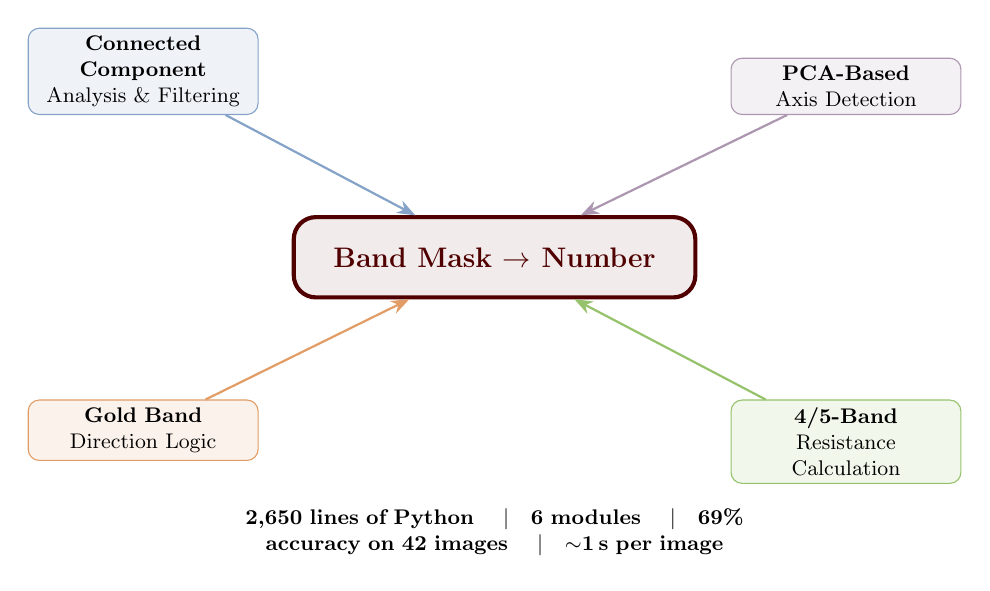
\begin{tikzpicture}[scale=0.85, transform shape]
  % Central block
  \node[rectangle, rounded corners=8pt, draw=tamumaroon, fill=tamumaroon!8,
    line width=1.5pt, minimum width=6cm, minimum height=1.2cm,
    font=\large\bfseries, text=tamumaroon] (center)
    {Band Mask $\rightarrow$ Number};

  % Surrounding items
  \node[rectangle, rounded corners=4pt, draw=pipeblue!60, fill=pipeblue!8,
    font=\small, text width=3.2cm, align=center, above left=1.5cm and 0.5cm of center]
    (a1) {\textbf{Connected Component}\\Analysis \& Filtering};

  \node[rectangle, rounded corners=4pt, draw=pipepurple!60, fill=pipepurple!8,
    font=\small, text width=3.2cm, align=center, above right=1.5cm and 0.5cm of center]
    (a2) {\textbf{PCA-Based}\\Axis Detection};

  \node[rectangle, rounded corners=4pt, draw=pipeorange!60, fill=pipeorange!8,
    font=\small, text width=3.2cm, align=center, below left=1.5cm and 0.5cm of center]
    (a3) {\textbf{Gold Band}\\Direction Logic};

  \node[rectangle, rounded corners=4pt, draw=pipegreen!60, fill=pipegreen!8,
    font=\small, text width=3.2cm, align=center, below right=1.5cm and 0.5cm of center]
    (a4) {\textbf{4/5-Band}\\Resistance Calculation};

  \draw[-{Stealth}, pipeblue!60, thick] (a1) -- (center);
  \draw[-{Stealth}, pipepurple!60, thick] (a2) -- (center);
  \draw[-{Stealth}, pipeorange!60, thick] (a3) -- (center);
  \draw[-{Stealth}, pipegreen!60, thick] (a4) -- (center);

  % Stats
  \node[below=3cm of center, font=\small, text width=12cm, align=center] {
    \textbf{2,650 lines of Python} \quad$|$\quad
    \textbf{6 modules} \quad$|$\quad
    \textbf{69\% accuracy on 42 images} \quad$|$\quad
    \textbf{$\sim$1\,s per image}
  };
\end{tikzpicture}
\end{center}
\end{frame}

% ---- SLIDE: Thank You ----
{
\setbeamertemplate{footline}{}
\begin{frame}{}
\vfill
\begin{center}
{\Huge\bfseries\color{tamumaroon} Thank You}

\vspace{0.5cm}
{\large Questions?}

\vspace{1cm}
{\small
ECEN 491 --- Undergraduate Research\\
Texas A\&M University at Qatar\\
Fall 2025
}
\end{center}
\vfill
\end{frame}
}

\end{document}
